\documentclass{article}[12pt,a4paper]
\usepackage{a4wide}
%\usepackage{fullpage}
\usepackage{tikz}
\usepackage{amssymb}
\usepackage{bbm}

\title{MA470 Assignment 2}
\author{Richard Douglas}
\date{February 4,  2014} %defaults to \today

\begin{document}
  \maketitle
  The final page of this submission consists of an appendix with derivations of general reusable results that 
  are used throughout my solutions. (Note that $d_\pm^*$ takes $q$ into account.)\newline
  \begin{enumerate}
  \item[\textbf{Exercise 2.1}] 
  (d) 
  $$\widetilde{P}(S^{\alpha}(T_2) > S^{\beta}(T_1)) = \widetilde{P}(\frac{S^{\alpha}(T_2)}{S^{\beta}(T_1)} > 1)$$
      
      Where 
      $$S^\alpha(T_2) = S^\alpha e^{\alpha(r - q -\sigma^2/2)T_2 + \alpha\sigma\widetilde{W}(T_2)}$$
      $$S^\beta(T_1) = S^\beta e^{\beta(r - q - \sigma^2/2)T_1 + \beta\sigma\widetilde{W}(T_1)}$$
      
      The probability is thus
      $$= \widetilde{P}(S^{\alpha - \beta}e^{(r - q - \sigma^2/2)(\alpha T_2 - \beta T_1) + 
       \sigma(\alpha\widetilde{W}(T_2) - \beta\widetilde{W}(T_1)) } > 1)$$
       
       \hfill (where
       $Var(\sigma(\alpha\widetilde{W}(T_2) - \beta\widetilde{W}(T_1)))
       = \sigma^2(\alpha^2T_2 + \beta^2T_1 - 2\alpha\beta T_1)$)
   
       $$= \widetilde{P}(\widetilde{Z} >  
       \frac{- (\alpha - \beta)ln(S) - (r - q - \sigma^2/2)(\alpha T_2 - \beta T_1)}
       { \sigma\sqrt{\alpha^2T_2 + \beta^2T_1 - 2\alpha\beta T_1}})$$
       
       $$= N(\frac{(\alpha - \beta)ln(S) +  (r - q - \sigma^2/2)(\alpha T_2 - \beta T_1)}
       {\sigma\sqrt{\alpha^2T_2 + \beta^2T_1 - 2\alpha\beta T_1}})$$ \newline
      
  (e) I assume that $T_2 > T_1 > t$. The other cases can be obtained by relabelling the time values.
  $$\widetilde{P}(S(T_2) > S(T_1) > S(t)) = 
  \widetilde{P}(\frac{S(T_2)}{S(T_1)} > 1 \mbox{ and } \frac{S(T_1)}{S(t)} > 1)
  = \widetilde{P}(\frac{S(T_2)}{S(T_1)} > 1) \cdot \widetilde{P}(\frac{S(T_1)}{S(t)} > 1)$$
  \hfill(because $\frac{S(T_2)}{S(T_1)}$ and $\frac{S(T_1)}{S(t)}$ are independent.)
  
  By \textbf{Result 1}, the desired probability is thus
  $$= N(d_-^*(1,T_2 - T_1)) \cdot N(d_-^*(1,T_1 - t))$$ \newline
  \pagebreak
  
  \item[\textbf{Exercise 2.1}]
  (f) $$\widetilde{P}(S(T_1) < K_1, S(T_2) > K_2)
  = \widetilde{P}(S(T_1) < K_1 \mbox{ and } S(T_2) > K_2)$$
  
  \textbf{Case $T_1 < T_2$:}
  $$ = \widetilde{P}(S(T_1) < K_1) \cdot \widetilde{P}(S(T_2) > K_2 | S(T_1) < K_1)$$
  $$
  = \widetilde{P}(S(T_1) < K_1) \cdot
  \int_0^{K_1}{\widetilde{P}(S(T_2) > K_2 | S(T_1) = s) ds}
  $$
  $$
  = \widetilde{P}(S(T_1) < K_1) \cdot \int_0^{K_1}{\widetilde{P}(\frac{S(T_2)}{S(T_1)} > \frac{K_2}{s})ds}
  $$
  By \textbf{Result 1} and \textbf{Result 2}
  $$
  =  (1 - N(d_-^*(S/K_1, T_1)) \cdot \int_0^{K_1}{N(d_-^*(s/K_2, T_2 - T_1))ds}
  $$
  \textbf{Case $T_2 < T_1$:}
  $$ = \widetilde{P}(S(T_2) > K_2) \cdot \widetilde{P}(S(T_1) < K_1 | S(T_2) > K_2)$$
  $$ = N(d_-^*(S/K_2, T_2)) \cdot \int_{K_2}^{\infty}{1 - N(d_-^*(s/K_1, T_1 - T_2))ds}$$ \newline
  
  \item[\textbf{Exercise 2.2}]
  (c)
  $$ V(t,S) = e^{-r\tau} \widetilde{E}_{t\mbox{,}S}\left[ a|S^{\alpha}(T) - K|\right]$$
  $$
  = a e^{-r\tau} (2\widetilde{E}_{t\mbox{,}S}\left[ (S^{\alpha}(T) - K)  
  \mathbbm{1}_{\{ S^\alpha(T) > K \}} \right]
  + \widetilde{E}_{t\mbox{,}S}\left[K - S^{\alpha}(T) \right])
  $$
  
  Where
  $$
   \widetilde{E}_{t\mbox{,}S}\left[K \right] = K
  $$
   $$
   \widetilde{E}_{t\mbox{,}S}\left[ S^{\alpha}(T) \right] =  S^\alpha e^{\alpha(r - q - \sigma^2(1  - \alpha)/2 )\tau}
  $$
  \hfill (by \textbf{Result 3})
  
  \textbf{Case $\alpha > 0$:}
  
  $$
  \widetilde{E}_{t\mbox{,}S} \left[ K \cdot \mathbbm{1}_{\{ S^\alpha(T) > K \}} \right]
  = K \cdot \widetilde{P}_{t\mbox{,}S}(S(T) > K^{1/\alpha})
  = K \cdot N(d_-^*(S/K^{1/\alpha}, \tau))
  $$
  \hfill (by \textbf{Result 1})
  
  $$
  \widetilde{E}_{t\mbox{,}S} \left[ S^{\alpha}(T) \cdot  \mathbbm{1}_{\{ S^\alpha(T) > K \}} \right] 
	  = S^\alpha e^{\alpha (r - q -\sigma^2/2) \tau} \cdot \widetilde{E} 
	  \left[ e^{\alpha\sigma\sqrt\tau \widetilde{Z}}  
	  \mathbbm{1}_{\{ \widetilde{Z} > -d_-^*(S/K^{1/\alpha}, \tau) \}} \right]
  $$
  $$
  = S^\alpha e^{\alpha (r - q - \sigma^2/2)\tau}\cdot e^{(\alpha\sigma)^2\tau/2} 
  (1 - N(-d_-^*(S/K^{1/\alpha}, \tau) - \alpha\sigma\sqrt\tau ))
  $$
  \hfill (by \textbf{Result 4})
  $$
    = S^\alpha e^{\alpha (r - q - \sigma^2(1 - \alpha)/2)\tau}
    \cdot N(d_-^*(S/K^{1/\alpha}, \tau) + \alpha\sigma\sqrt\tau )
  $$
  
  Therefore: 
  $$V(\tau, S) = ae^{-r\tau}(
  S^\alpha e^{\alpha (r - q - (1 - \alpha)\sigma^2/2)\tau} \cdot 
  (2 \cdot N(d_-^*(S/K^{1/\alpha}, \tau) + \alpha\sigma\sqrt\tau ) - 1)
  + K \cdot (2 \cdot N(d_-^*(S/K^{1/\alpha}, \tau))  - 1))$$ 
  
  
  \pagebreak
  \textbf{Case $\alpha < 0$:}
  
   $$
  \widetilde{E}_{t\mbox{,}S} \left[ K \mathbbm{1}_{\{ S^\alpha(T) > K \}} \right]
  = K \cdot \widetilde{P}_{t\mbox{,}S}(S(T) < K^{1/\alpha})
  = K \cdot (1 -  N(d_-(S/K^{1/\alpha}, \tau)))
  $$
  \hfill (by \textbf{Result 1})
  
  $$
  \widetilde{E}_{t\mbox{,}S} \left[ S^{\alpha}(T) \cdot  \mathbbm{1}_{\{ S^\alpha(T) > K \}} \right]
  =  S^\alpha e^{\alpha (r - q -\sigma^2/2) \tau} \cdot \widetilde{E} 
	  \left[ e^{\alpha\sigma\sqrt\tau \widetilde{Z}}  (1 - 
	  \mathbbm{1}_{\{ \widetilde{Z} > -d_-^*(S/K^{1/\alpha}, \tau) \}}) \right]
  $$
  
  $$
  = S^\alpha e^{\alpha (r - q -\sigma^2/2) \tau} \cdot 
  (e^{(\alpha\sigma)^2\tau/2} - e^{(\alpha\sigma)^2\tau/2} 
  (1 - N(-d_-^*(S/K^{1/\alpha}, \tau) - \alpha\sigma\sqrt\tau )))
  $$
  \hfill (by \textbf{Result 4})
  $$
    = S^\alpha e^{\alpha (r - q - \sigma^2(1 - \alpha)/2)\tau}
    \cdot (1 - N(d_-^*(S/K^{1/\alpha}, \tau) + \alpha\sigma\sqrt\tau ))
  $$
  
  Therefore:
  $$V(\tau, S) = ae^{-r\tau}(
  S^\alpha e^{\alpha (r - q - (1 - \alpha)\sigma^2/2)\tau} \cdot 
  (1 - 2 \cdot N(d_-^*(S/K^{1/\alpha}, \tau) + \alpha\sigma\sqrt\tau ))
  + K \cdot (1 - 2 \cdot N(d_-^*(S/K^{1/\alpha}, \tau))))$$ \newline
  
  \item[\textbf{Exercise 2.3}]
  (a)
   \begin{center}
   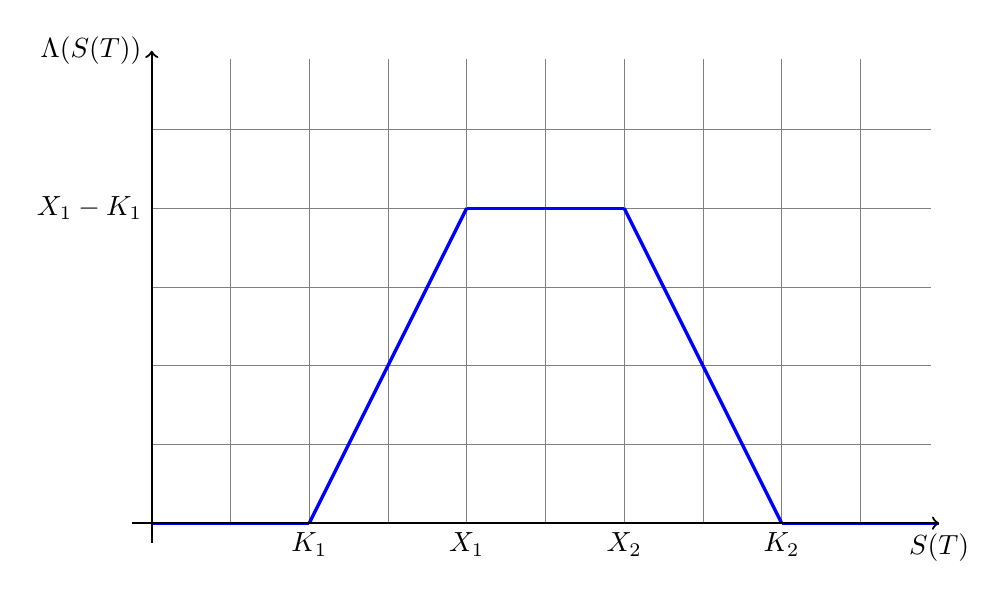
\begin{tikzpicture}[domain=0:8, align=center]
     \draw[very thin, color=gray](0,0) grid(9.9,5.9);
     
    \draw (2,0) node[below] {$K_1$};
    \draw (4,0) node[below] {$X_1$};
    \draw (6,0) node[below] {$X_2$};
    \draw (8,0) node[below] {$K_2$};
    \draw (0,4) node[left] {$X_1 - K_1$}; 
     
     \draw[very thick, color=blue] (0,0) -- (2,0);
     \draw[very thick, color=blue] (2,0) -- (4,4);
     \draw[very thick, color=blue] (4,4) -- (6,4);
     \draw[very thick, color=blue] (6,4) -- (8,0);
     \draw[very thick, color=blue] (8,0) -- (10,0);
     
     \draw[thick, ->] (-0.25,0) -- (10,0) node[below]{$S(T)$};
     \draw[thick, ->] (0,-0.25) -- (0,6) node[left]{$\Lambda(S(T))$};
   \end{tikzpicture}
   \end{center}
   \hfill (strike values not necessarily evenly spaced out.)
   
   This European option can be replicated by purchasing a European call with strike $K_1$,
   writing a European call with strike $X_1$, purchasing a European call with strike $K_2$,
   and writing a European call with strike $X_2$. \newline
  
  (b) Using the fact that
  $$C(\tau, S, K, \sigma, r, q) = e^{-q\tau}C(\tau, S, K, \sigma, r-q, 0)$$
  The value of the portfolio is
  $$V(\tau, S, \sigma, r, q, K_1, X_1, K_2, X_2) = 
  C(\tau, S, K_1, \sigma, r, q) - C(\tau, S, X_1, \sigma, r, q)
  + C(\tau, S, K_2, \sigma, r, q) - C(\tau, S, X_2, \sigma, r, q)$$
  
  $$= e^{-q\tau}( C(\tau, S, K_1, \sigma, r-q, 0) - C(\tau, S, X_1, \sigma, r-q, 0)
  + C(\tau, S, K_2, \sigma, r-q, 0) - C(\tau, S, X_2, \sigma, r-q, 0))$$
  
  $$
  = Se^{-q\tau}(N(d_+^*(S/K_1,\tau)) -  N(d_+^*(S/X_1,\tau)) 
  +  N(d_+^*(S/K_2,\tau)) -  N(d_+^*(S/X_2,\tau))) 
  $$
  $$
   - e^{-r\tau}(K_1 \cdot N(d_-^*(S/K_1,\tau)) - X_1 \cdot N(d_-^*(S/X_1,\tau)) 
  + K_2 \cdot N(d_-^*(S/K_2,\tau)) - X_2 \cdot N(d_-^*(S/X_2,\tau)))
  $$ \newline
  
  (c) Using the following fact about hedging European calls
  $$\Delta_C(t,S;r,q) = e^{-q\tau}\Delta_C(t,S;r - q, 0)$$
  And letting $\Delta_K(t,S;r,q)$ be the delta position for a European call with strike $K$,
  The desired delta position is
  $$\Delta(t,S;r,q) = \Delta_{K_1}(t,S;r,q) - \Delta_{X_1}(t,S;r,q) + \Delta_{K_2}(t,S;r,q) - \Delta_{X_2}(t,S;r,q)$$
  $$= e^{-q\tau}(N(d_+^*(S/K_1,\tau)) - N(d_+^*(S/X_1,\tau)) + N(d_+^*(S/K_2,\tau)) - N(d_+^*(S/X_2,\tau)))$$ \newline
  
  \textbf{Important:} $d_\pm^*(m,\tau)$ is defined in the appendix and is slightly different from the function in the
  lecture notes in that it takes q into consideration. \newline
  
  
  \item[\textbf{Exercise 2.4}]
  (a)
  $$ V(t,S) = e^{-r\tau} \widetilde{E}_{t\mbox{,}S}\left[ \Sigma_{n = 0}^N{a_nS^n(T)} \right]
  =  e^{-r\tau}(a_0 + \Sigma_{n = 1}^N{a_n \widetilde{E}_{t\mbox{,}S}\left[S^n(T) \right]})$$
  
  By \textbf{Result 3} this is
  $$= e^{-r\tau}(a_0 + \Sigma_{n = 1}^N{a_n S^n e^{n(r - q - \sigma^2(1  - n)/2 )\tau}})$$
  Or more compactly
  $$= e^{-r\tau}(a_0 + \Sigma_{n = 1}^N{a_n \Theta^n}e^{(n\sigma)^2\tau/2})$$
  \hfill (where $\Theta := Se^{(r - q - \sigma^2/2)\tau}$)
  
  \end{enumerate}
  \pagebreak
  \section*{Appendix}
  Throughout this assignment I make use of
  $$d_{\pm}^{*}(m,\tau) := \frac{ln(m) + (r - q \pm \sigma^2/2)\tau}{\sigma\sqrt\tau}$$
  which is different from the usual definition since it takes the continuous dividend yield $q$ into account. \newline
  \newline\textbf{Result 1:}
  $$\widetilde{P}(\frac{S(T)}{S(t)} > \frac{K}{S}) = 
  \widetilde{P}(\widetilde{Z} > \frac{-ln(S/K) - (r - q - \sigma^2/2)(T - t)}{\sigma\sqrt{T - t}}) = N(d^*_-(S/K,T - t))$$ \newline
  \textbf{Result 2:}
  $$\widetilde{P}(S(t) > K) = \widetilde{P}(\frac{S(t)}{S(0)} > \frac{K}{S(0)}) = N(d_-^*(S(0)/K,t))$$ \newline
  \textbf{Result 3:}
  $$\widetilde{E}_{t\mbox{,}S}\left[ S^{\alpha}(T) \right] = 
   S(t)^\alpha e^{\alpha(r - q - \sigma^2/2)\tau} \widetilde{E}\left[ e^{\alpha \sigma \sqrt\tau \widetilde{Z}}\right] =
    S(t)^\alpha e^{\alpha(r - q - \sigma^2(1  - \alpha)/2 )\tau}$$ 
    \textbf{Result 4:}
    $$
    E \left[ e^{aZ} \mathbbm{1}_{\{ Z > b \}} \right] = 
    \int_b^{\infty} { e^{az} \frac{1}{\sqrt{2\pi}} e^{-z^2/2} dz} = 
    e^{a^2/2}\int_{b}^{\infty}{\frac{1}{\sqrt{2\pi}}  e^{-(z - a)^2/2} dz} = 
     e^{a^2/2} \cdot (1 - N(b - a))
    $$
  
\end{document}